\documentclass[11pt,numberedappendix,twocolappendix,]{emulateapj}


\usepackage{natbib}
\usepackage{amsmath}
\usepackage{amssymb}
\usepackage{aas_macros}
\usepackage{appendix}
\usepackage{multirow}
\usepackage{color,xcolor}
\usepackage{url}
\usepackage{hyperref}
\hypersetup{colorlinks,linkcolor={blue!50!black},citecolor={blue!50!black},urlcolor={blue!50!black}}

\bibliographystyle{apj}

\renewcommand{\bibname}{References}

\def\water{H$_2$O }
\def\preslevel{2.47}
\def\modelE{{\it ROCKE-3D}}
\def\CHHHH{CH$_4$}
\def\COO{CO$_2$}
\def\COO{CO$_2$}
\def\memo#1{\color{red}$[${\bf #1}$]$ \color{black}}

\def\Rp{R_{\rm p}}
\def\Rtransit{R_{\rm transit}}
\def\OD#1#2{\frac{d#1}{d#2}}
\def\PD#1#2{\frac{\partial #1}{\partial #2}}

%%%%%%%%%%%%%%%%%%%%%%%%%%%%%%%%%%%%%%%%%%%%%%%%%%%%%%%%%%%%%%%%%%%
\shorttitle{Water Vapor in Upper Atmospheres of Temperate Terrestrial Exoplanets}
\shortauthors{Fujii et al.}

%%%%%%%%%%%%%%%%%%%%%%%%%%%%%%%%%%%%%%%%%%%%%%%%%%%%%%%%%%%%%%%%%%%
\begin{document}

%%%%%%%%%%%%%%%%%%%%%%%%%%%%%%%%%%%%%%%%%%%%%%%%%%%%%%%%%%%%%%%%%%%
\title{Modeling of Water Vapor in the Upper Atmospheres of 
\\Temperate Earth-size Planets}
\author{Yuka Fujii}
\affil{NPP fellow, Universities Space Research Association}
\affil{Goddard Institute for Space Studies, 2880 Broadway, New York, NY}
\affil{Earth-Life Science Institute, Tokyo Institute of Technology, Ookayama, Meguro, Tokyo 152-8550, Japan}
\author{Anthony D. Del Genio}
\author{David S. Amundsen}
\affil{Goddard Institute for Space Studies, 2880 Broadway, New York, NY}

%%%%%%%%%%%%%%%%%%%%%%%%%%%%%%%%%%%%%%%%%%%%%%%%%%%%%%%%%%%%%%%%%%%
\begin{abstract}

\water is a key molecule in characterizing atmospheres of temperate terrestrial planets, and the observations of transmission spectra are expected to play a primary role in detecting its signatures in the near future. 
%
Detectability of \water absorption features in transmission spectra primarily depends on the mixing ratio of \water in the upper part of the atmosphere. 
%
While the stratospheric \water mixing ratio of the Earth is as low as $10^{-6}$ due to the cold trap, the efficiency of the cold trap depends on the atmospheric properties. 
%
Here we study the 3-dimensional distributions of \water for synchronously rotating aqua planets using the GCM, \modelE, and examine the effect of the incident star spectra. 
%
We observe a gradual increase of \water mixing ratio in response to the increased incident flux, while the surface temperature around the substellar point is moderate. 
%
At higher incident flux, we find a large-scale circulation in the upper part of the atmosphere, presumably originating from the high heating rate due to the enhanced absorption by abundant \water in the upper atmosphere. 
%
The interplay between the efficient vertical transport of \water by this large-scale circulation and the radiative heating rate appears to play the key role in determining the steady state of the \water mixing ratio in the upper atmosphere.  
%
Consistently, \water is found to be in a good correlation with the near-infrared portion of the incident flux. 
%
Our results imply that various levels of \water mixing ratios in the upper atmosphere may be expected for synchronously rotating temperate terrestrial planets, and for the favorable ones the \water absorption features in the transmission spectra are increased by factor of a few, loosening the observational demands. 
%
\end{abstract}
%%%%%%%%%%%%%%%%%%%%%%%%%%%%%%%%%%%%%%%%%%%%%%%%%%%%%%%%%%%%%%%%%%%


%%%%%%%%%%%%%%%%%%%%%%%%%%%%%%%%%%%%%%%%%%%%%%%%%%%%%%%%%%%%%%%%%%%
\keywords{exoplanet, atmosphere}

%%%%%%%%%%%%%%%%%%%%%%%%%%%%%%%%%%%%%%%%%%%%%%%%%%%%%%%%%%%%%%%%%%%
\section{Introduction}
\label{s:intro}

One of the primary interests in future observations of Earth-size planets is the presence of \water. 
Knowing what kind of planets harbor it and what do not is an essential ingredient to assess the origin of planetary \water, or constraining the evolutional pathway. 
It also serve as the important prior knowledge to prioritize the targets for identifying biosignatures, on the assumption that \water is a prerequisite for life as know it. 

Nevertheless, it has been pointed out that detecting molecular signatures on terrestrial planets is challenging \citep{Cowan2015}. 
Earth-size planets are indeed small and the atmospheres are presumably thin, making atmospheric features in transit spectra typically at the order of ppm. 
This requires a significant devotion of telescopes, even in the case where the observational noise is limited by stellar photon noise. 
\water is particularly difficult because, while \water is a dominant opacity source of Earth's atmosphere, mixing ratio of \water above the troposphere---where the transmission spectroscopy typically probes---is fairly small due to the ``cold trap'', i.e., water vapor evaporated from the surface is transported upward, but up in the atmosphere water condenses and most of it precipitates, leaving the stratosphere fairly dry. 
Several studies of modeling transmission spectra of the Earth found the signatures undesirebly weak signatures of the Earth \citep[e.g.,][]{Ehrenreich2006, Kaltenegger2009, Betremieux2013, Misra2014}. 
However, the efficiency of the cold trap depends on the atmospheric properties in general. 

The mixing ratio in the stratosphere is also closely related to planetary water loss and thus planetary habitability. 
\citet{Kasting1993} considered the maximum mixing ratio that allow for a planet to sustain Earth-mass water within Earth age, $\sim 3 \times 10^{-3}$, as a criterion for the inner edge of the habitable zones (the threshold for the moist-greenhouse stage). 
Motivated mainly by this ``habitability'' aspect, atmospheric models with different levels of complexity have examined the stratospheric \water with varying planetary properties, or equivalently the efficiency of the cold trap. 

\citet{Kasting1993} and \citet{Kopparapu2013} used a simple 1D model with saturated troposphere and isothermal stratosphere to examine the response of the stratospheric \water mixing ratio to the increased instellation. 
% 
\citet{Wordsworth2013} used 1D radiative-convective models with different atmospheric compositions and found that in some range of parameters the efficiency of the cold trap is smaller than the Earth, which could lead to a significant loss of water. 
%
\citet{Rugheimer2013} and \citet{Rugheimer2015} combined 1D radiative-convective model with photochemical model to assess the effect of spectral energy distribution of the incident stellar spectra on atmospheric profiles, and observed an enhanced water mixing ratio in the stratosphere for planet around late-type stars (while not discussed in detail). 

Inevitably, 1D models rely on several assumptions that cannot be solved within the model, including the global transport of heat and water vapor as well as the effect of clouds. 
Over several years, various 3-dimensional global circulation models (GCMs) revisited the atmospheric profile of terrestrial planets and have demonstrated the importance of taking account of the 3-dimensional circulation and climate heterogeneity. 

% Abe
 \citet{Abe2011} performed a series of GCM experiments using the atmospheric general circulation model 5.4g from the Center for Climate System Research, the University of Tokyo, and pointed out that dry planets with limited amount of water have stable climate over the wider range of orbital distance. 
% Leconte
\citet{Leconte2013b}, using the Laboratoire de M\'et\'eorologie Dynamique (LMD) generic climate model from France, and 
% Wolf
\citet{Wolf2014, Wolf2015}, using the Community Atmosphere Model version 3 and 4 from the National Center for Atmospheric Research, found that with 3-dimensional model is more resistant against the increased instellation and have modest surface temperature and low stratospheric water vapor with wider range of instellation than what 1D models predict. This is primarily due to the unsaturated subsident region of the Hadley cell, which was not taken into account in 1D models. 

The 3-dimensional climate is drastically different for habitable-zone planets around late-type stars not only due to the difference on the spectral energy distribution of the star but also because they are likely to be synchronously rotating \memo{paper to cite?}. 
%
\citet{Yang2013} pointed out that for tidally-locked planets, the strong convection around the sub-stellar point produces thick clouds which contribute to keep the surface temperature moderate for a much wider range of in stellation; see also \citet{Yang2014,Way2015,Kopparapu2016}. 
They primarily studied the highest instellation that allows for the model to converge as the proxy for the inner edge. 
While they also presented the stratospheric water vapor, the discussion was limited. 

Motivated by these works on the stabilized climate of planets around late-type stars, we are particularly interested in the water vapor transport  into the upper atmosphere, not only because it affects the water loss rate (and thus conventional criterion for habitable condition) but also because it limits our ability to detect \water through the transmission spectroscopy. 
%
Indeed, the planets around later type stars are best suited for future transit observations for several reasons including the higher transit probability, larger signals in transmission spectra, and the abundance of the late-type stars in the nearby universe. 

%The water mixing ratio in the stratosphere of a planet around late-type stars has been controversial and not been fully understood \memo{OK...?}. 
%Some of the 1D atmospheric models \citep{Rugheimer2013, Rugheimer2015} as well as 3D models \citep{Godolt2015} infer orders of magnitude larger water vapor mixing ratio in the stratosphere on planets around late-type stars with similar instellation as the Earth receives, 
%while other 3D GCM models show stratospheric mixing ratio of order of $10^{-6}$ even for planets around M-type stars. 

In order to obtain better insights into the processes that controls water vapor mixing ratio in the upper atmospheres where transit observations probe, we conduct series of experiments with Global Circulation Model \modelE \ for planets which receive similar amount of energy from the host star to the Earth's. 
\modelE \ solves the atmospheric dynamics and radiative fields up to $0.1$ mbar ($\sim $70-80 km), to be able to sufficiently resolve the stratosphere. 
We particularly study the dependence of water vapor mixing ratio on the incident flux (total incident flux and the spectral type), fixing planetary parameters (radius, gravity, atmospheric composition, and atmospheric pressure), so as to separate the effect of each parameter. 

We also present mock transmission spectra based on GCM outputs in order to evaluate the detectability of \water signatures with future transmission spectroscopy using e.g. JWST, or next-generation ground-based telescopes. 




%%%%%%%%%%%%%%%%%%%%%%%%%%%%%%%%%%%%%%%%%%%%%%%%%%%%%%%%%%%%%%%%%%%
\section{Model}

%%%%%%%%%%%%%%%%%%%%%%%%%%%%%%%%%%%%%%%%%%%%
\subsection{GCM experiments}
%%%%%%%%%%%%%%%%%%%%%%%%%%%%%%%%%%%%%%%%%%%%

%%%%%%%%%%%%%%%%%%%%%%%%%%%%%%%%%%%
\begin{figure}[!bh]
    \begin{center}
    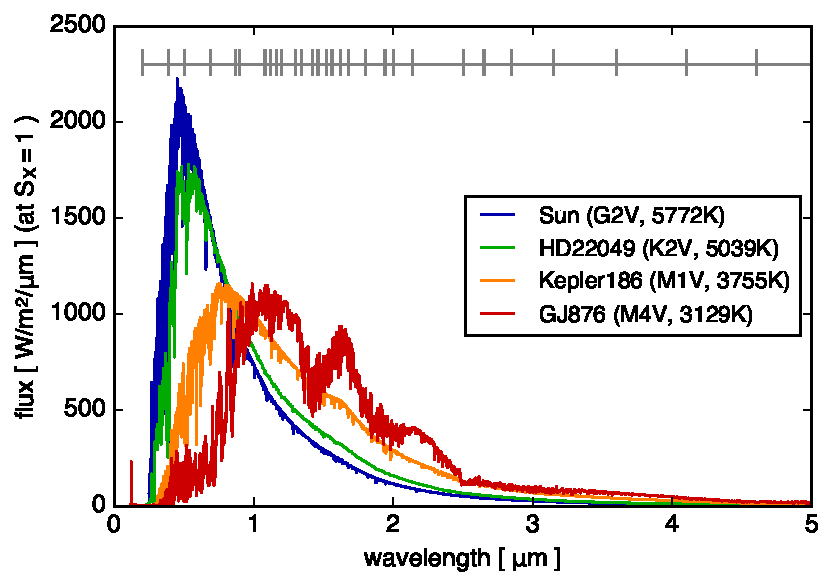
\includegraphics[width=\hsize]{fig/star_spectra.pdf}
    \end{center}
\caption{The spectra of the stars considered in this paper. The flux is normalized so that the total incident flux matches the solar constant. The resolution is lowered for display purposes, but higher resolution spectra were used to calculate the correlated-k table weighted by the stellar spectrum. The data sources are \citet{Kurucz1995} (Sun), \citet{Segura2003} (HD 22049), \memo{?} (Kepler-186), and \citet{Domagal-Goldman2014} (GJ876). \memo{what kind of resolution would be relevant?}}
\label{fig:star_spectra}
\end{figure}
%%%%%%%%%%%%%%%%%%%%%%%%%%%%%%%%%%%

We use a 3-dimensional GCM named {\it ROCKE-3D} \citep{way2016,ROCKE3D} \memo{cite  the ROCKE-3D paper}. 
This is a generalization from the GCM called {\it ModelE2} \citep{Schmidt2014}, which has been developed for the Earth at NASA's Goddard Institute for Space Studies. 
The basic architecture of ROCKE-3D is same as the version used by \citet{way2016}, but the radiation module has been replaced by UK Met Office's {\it Socrates} \citep{Edwards1996} after the paper was published. 
{\it Socrates} utilizes the correlated-k method to compute radiative transfer. 
We used 6 and 9 bands for short wave and long wave, respectively. 
We paid special attention to the accuracy of the radiative transfer because the radiation scheme specialized for the Earth system may no longer be accurate when we change the spectral types of the star and/or \water mixing ratio becomes extreme (see the result section below). 
We check the accuracy of the radiation by comparing the radiation calculation in the GCM with the higher-resolution calculations, and found the reasonable match;  see Appendix \ref{ap:radiation} for more details. 

The model was configured to have horizontal grids with 4 degree resolution in latitude and 5 degree resolution in longitude, and 40 vertical layers covering up to 0.14 mbar (corresponding to $\sim 60$ km in the case of the Earth). 

We consider synchronously rotating planets for the relevance to the future transmission observations of close-in systems \memo{mention the possibility of non-synchronously rotating situation?}. 
We consider aqua planets, i.e., the planets are wholly covered with water. 
As for the treatment of ocean, we considered q-flux ocean with 900 m deoth for the fiducial runs for simplicity. However, in Section \ref{ss:sensitivity_ocean} we also show the results of the runs with fully dynamic ocean, to quantify the sensitivity of the results to the assumption of ocean. 

Our atmosphere is 1 bar N$_2$-dominated atmosphere with 1 ppm CO$_2$, to match the assumption of \citet{Kopparapu2016}. 

In our experiments, we mainly changed two parameters: the total incident flux normalized by the solar constant, $S_X$, and the spectral types of the star. 
For the latter, four types of stars are considered: Sun (G2V; 5776K), HD 22049 \citep[][K2V, 5084K, $0.82M_{\odot }$, $0.73R_{\odot }$]{Segura2003}, Kepler-186 \citep[][M1V, 3755K, $0.54M_{\odot }$, $0.52R_{\odot }$]{}\memo{need to ask Nancy who should be cited for Kepler-186}, and GJ876 \citep[][M4V, 3473K, $0.334M_{\odot }$, $0.36R_{\odot }$]{Domagal-Goldman2014}. 
These four spectra are shown in Figure \ref{fig:star_spectra}. 

The orbital period (= spin period) is changed according to the Kepler's 3rd law, to be consistent with the total incident flux the planet receives and the stellar mass. While the incident flux and the orbital period are changed simultaneously for the fiducial runs, we also isolate the effect of the orbital period in Section \ref{ss:sensitivity_Porbit}. 


%%%%%%%%%%%%%%%%%%%%%%%%%%%%%%%%%%%%%%%%%%%%
\subsection{Simulation of transmission spectra}
%%%%%%%%%%%%%%%%%%%%%%%%%%%%%%%%%%%%%%%%%%%%

We also simulate transmission spectra based on the outputs of GCM experiments, as it were observed in a transiting geometry. 
We obtain the vertical profile of atmosphere (temperature, water vapor, and cloud particles) along the ``limb'' by linearly interpolating the profiles of the GCM grid points adjacent to the limb. 
(The ``limb'' corresponds to the boundary between the dayside and the nightside, in other words a great circle that passes $\pm 90^{\circ} $ longitude measured from the substellar point.)

We trace the optical paths of the transmitted ray taking account of the refraction due to the atmosphere, according to \citet{vanderWerf2008}, following \citet{Misra2014}. 
We compute the spectral opacity at different points along the path, considering Rayleigh scattering and the absorption by atmospheric profiles \memo{and clouds?}. 
We did not incorporate multiple scattering of atmospheres. 

In computing the absorption by atmospheric molecules, we use high-resolution line-by-line opacity tables based on HITRAN 2012 database \citep{Rothman2013}, prepared seperately from the correlated-k opacity used in the GCM. 
Each line in the HITRAN 2012 database is convolved with the voigt profile which takes account of Lorentzian pressure broadening and Doppler broadening, 
and the cross sections are computed at varying pressures and temperatures, with a constant interval of the wavenumber grids : $\Delta k = 1\,{\rm cm}^{-1}$. 
The pressure and temperature grids are $P = \{10^{-5},\, 10^{-4},\,...,\,10^3\}$ mbar and $T = \{100,\, 150,\,...,\, 400\}$ K. 
The cross section at a particular altitude in the planetary atmosphere is obtained by interpolating the values at these lattice points. 


%%%%%%%%%%%%%%%%%%%%%%%%%%%%%%%%%%%%%%%%%%%%%%%%%%%%%%%%%%%%%%%%%%%
\section{Results}
\label{s:results}
%%%%%%%%%%%%%%%%%%%%%%%%%%%%%%%%%%%%%%%%%%%%%%%%%%%%%%%%%%%%%%%%%%%

%%%%%%%%%%%%%%%%%%%%%%%%%%%%%%%%%%%%%%%%%%%%
\subsection{General Trend in 3D Atmospheric Profiles}
\label{ss:result_H2Omixingratio}
%%%%%%%%%%%%%%%%%%%%%%%%%%%%%%%%%%%%%%%%%%%%

Before examining the dependence of the \water mixing ratio in the upper atmosphere, we shall show the 3-dimensional profiles of temperature and water vapor, in particular at which altitude the mixing ratio of the \water becomes relatively uniform, to identify what kind of \water mixing ratio can be regarded as a representative of the humidity in the upper atmosphere. 

Figures \ref{fig:3Dprofile_equator_GJ876} and \ref{fig:3Dprofile_equator_Sun} exhibit the profiles of temperature and \water mixing ratio along the equator  for GJ876 (M4V) and the Sun (G2V), respectively.  
In all panels, substellar point corresponds to the longitude of $-180^{\circ }$. 
In general, temperature and \water mixing ratio strongly depend on the distance from the substellar point near the surface, but is fairly uniform in the upper part of the atmosphere above 1 mbar, which is 40-50 km depending on the atmospheric temperature profiles. 
In all of the runs introduced below, the spatial variation of the \water mixing ratio above ?? mbar is within ??\% \memo{will be filled later based on dynamic ocean runs}. 
Indeed the cloud content in these layers is typically on the oder of $10^{-6} $ [kg/kg], and the residence time is \memo{describe better why it is uniform.}

Therefore, in the following, we use \water mixing ratio at \preslevel mbar as a representative of \water in the upper atmosphere. 

%%%%%%%%%%%%%%%%%%%%%%%%%%%%%%%%%%%
\begin{figure}[!hbt]
    \begin{minipage}{0.48\hsize}
    \begin{center}
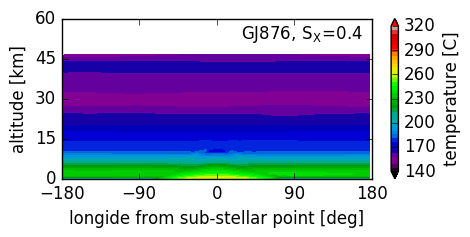
\includegraphics[width=\hsize]{fig/ANN0109-0134aijlAqOH0TLS_GJ876S04P48L40Q_temp.png}
    \end{center}
     \end{minipage}
  \begin{minipage}{0.48\hsize}
    \begin{center}
    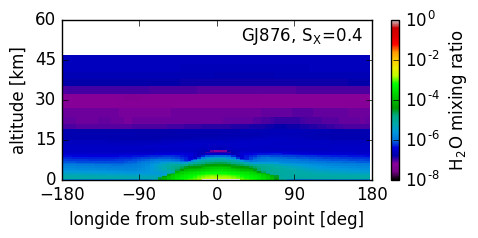
\includegraphics[width=\hsize]{fig/ANN0109-0134aijlAqOH0TLS_GJ876S04P48L40Q_xH2O.png}
    \end{center}
\end{minipage}
    \begin{minipage}{0.48\hsize}
    \begin{center}
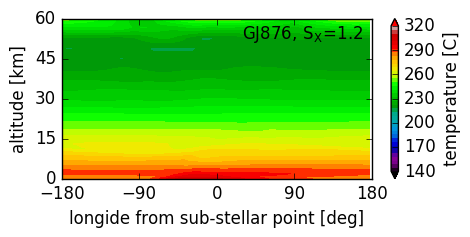
\includegraphics[width=\hsize]{fig/ANN0231-0287aijlAqOH0TLS_GJ876S12P21L40Q_temp.png}
    \end{center}
     \end{minipage}
  \begin{minipage}{0.48\hsize}
    \begin{center}
    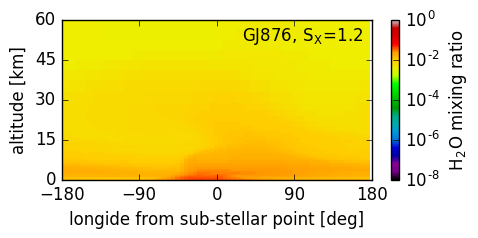
\includegraphics[width=\hsize]{fig/ANN0231-0287aijlAqOH0TLS_GJ876S12P21L40Q_xH2O.png}
    \end{center}
\end{minipage}
    \caption{Profiles of temperature and \water mixing ratio along the equator, for GJ876 (a M4V star). The blank area near the top is above the model top that is  0.14 mbar. \memo{will be replaced by the results of dynamic ocean.}}
\label{fig:3Dprofile_equator_GJ876}
\end{figure}
%%%%%%%%%%%%%%%%%%%%%%%%%%%%%%%%%%%


%%%%%%%%%%%%%%%%%%%%%%%%%%%%%%%%%%%
\begin{figure}[!hbt]
  \begin{minipage}{0.48\hsize}
    \begin{center}
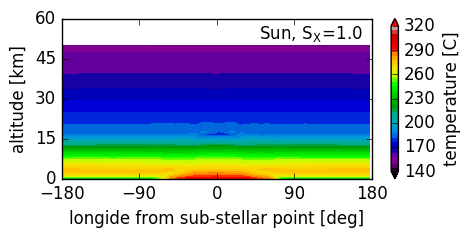
\includegraphics[width=\hsize]{fig/ANN0007-0010aijlAqOH0TLS_SunS10P365L40Q_temp.png}
    \end{center}
 \end{minipage}
   \begin{minipage}{0.48\hsize}
    \begin{center}
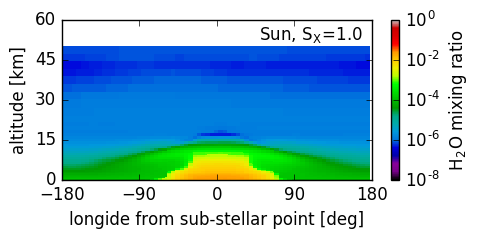
\includegraphics[width=\hsize]{fig/ANN0007-0010aijlAqOH0TLS_SunS10P365L40Q_xH2O.png}
    \end{center}
 \end{minipage}
  \begin{minipage}{0.48\hsize}
    \begin{center}
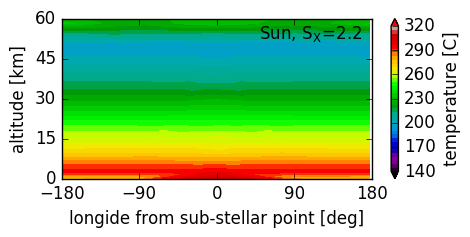
\includegraphics[width=\hsize]{fig/ANN0006-0012aijlAqOH0TLS_SunS22P202L40Q_temp.png}
    \end{center}
 \end{minipage}
   \begin{minipage}{0.48\hsize}
    \begin{center}
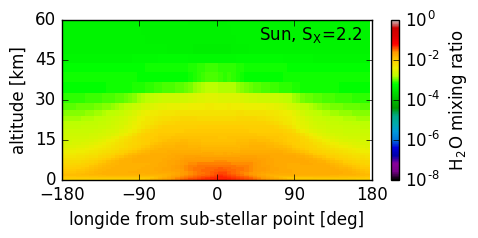
\includegraphics[width=\hsize]{fig/ANN0006-0012aijlAqOH0TLS_SunS22P202L40Q_xH2O.png}
    \end{center}
 \end{minipage}
    \caption{Same as \ref{fig:3Dprofile_equator_GJ876} but for a planet around the Sun.}
\label{fig:3Dprofile_equator_Sun}
\end{figure}
%%%%%%%%%%%%%%%%%%%%%%%%%%%%%%%%%%%

We also observe the optically thick clouds around the sub-stellar point as well as an increase of planetary albedo as a function of total incident flux (not shown in figures), consistently with \citet{Yang2013,Yang2014}, and \citet{Way2016}. 
This indicates the climate-stabilizing effect of clouds, having a negative feedback for the surface temperature, which is pointed out by \citet{Yang2013}. 
As shown in Figures \ref{fig:3Dprofile_equator_GJ876} and \ref{fig:3Dprofile_equator_Sun}, the maximum surface temperature does not exceed 320 K even in extreme cases in our experiments, where specific humidity is as high as $10^{-3}$; we will discuss this in the subsequent sections. 


%%%%%%%%%%%%%%%%%%%%%%%%%%%%%%%%%%%%%%%%%%%%
\subsection{Response of \water Mixing Ratio to Increased Incident Flux}
\label{ss:result_H2Omixingratio}
%%%%%%%%%%%%%%%%%%%%%%%%%%%%%%%%%%%%%%%%%%%%


%%%%%%%%%%%%%%%%%%%%%%%%%%%%%%%%%%%
\begin{figure}[!h]
    \begin{center}
    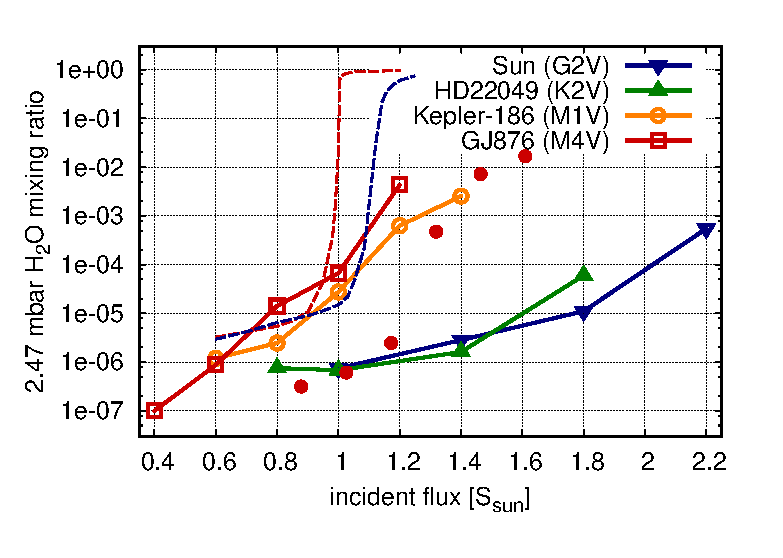
\includegraphics[width=\hsize]{fig/AqOH0TLS_xH2O_3mbar_all.eps}
    \end{center}
\caption{Water mixing ratio at \preslevel mbar as a function of total incident flux. The colors represent the stellar types: Sun (navy), HD22048 (green), Kepler-186 (orange), and GJ876 (red). \memo{TO BE REVISED}}                                                                                                             
\label{fig:xH2O_S0X}
\end{figure}
%%%%%%%%%%%%%%%%%%%%%%%%%%%%%%%%%%%

%%%%%%%%%%%%%%%%%%%%%%%%%%%%%%%%%%%
\begin{figure}[!h]
    \begin{center}
    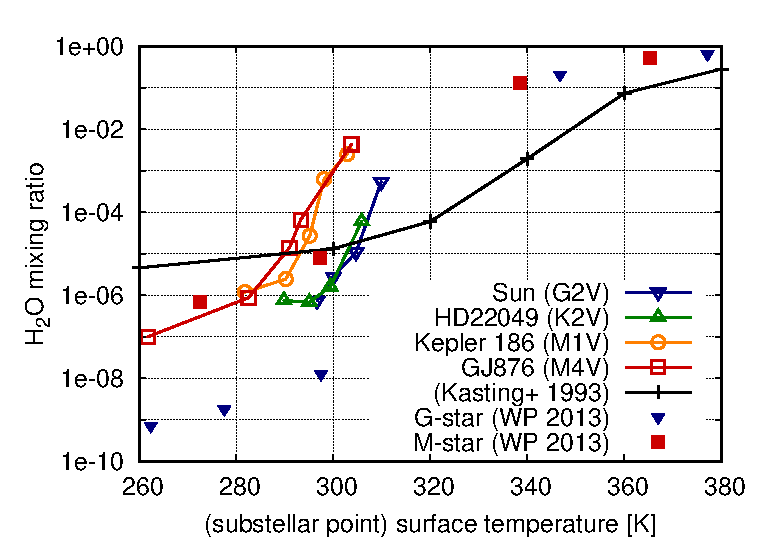
\includegraphics[width=\hsize]{fig/AqOH0TLS_tsurf_xH2O_GCM_Kasting_WP.eps}
    \end{center}
\caption{Water mixing ratio at \preslevel mbar as a function of the surface temperature around the sub-stellar point. \memo{TO BE REVISED}}                                                                                                             
\label{fig:AqOH0TLS_tsurf_xH2O_GCM_Kasting_WP}
\end{figure}
%%%%%%%%%%%%%%%%%%%%%%%%%%%%%%%%%%%

In this section, we examine in more detail how \water mixing ratio in the upper atmosphere depends on the incident flux (the total flux plus the spectral distribution) when other parameters are fixed. 

Figure \ref{fig:xH2O_S0X} presents \water mixing ratio at \preslevel ~mbar versus the total incident flux, $S_X$. 
Overall, we find a gradual increase of \water mixing ratio as a function of the total incident flux. 
The slope is much more gradual than suggested by 1D models, in particular those  of \citet{Kasting1993} and \citet{Wordsworth2013} with small $CO_2$ mixing ratio, which typically predict a rapid transition from an Earth-like dry stratosphere to  \water-dominated atmosphere. 
Our result that \water mixing ratio more slowly responds to the incident flux is qualitatively consistent with \citet{Yang2013} who studied synchronously rotating planets around of M-type and K-type stars using CAM3 with an emphasis on the stability of the climate. 
Note that we cannot directly compare with their results as the assumptions do not match perfectly; specifically, \cite{Yang2013} assumed a super-Earth with larger radius ($R=2R_{\oplus}$) and higher gravity ($g=1.4g_{\oplus}$), a N$_2$-dominated atmsphere with 400 ppm of CO$_2$, and the 60-days orbital period. 
The dependence on these other planetary parameters will be investigated in the future. 

Because these are synchronously rotating planets which form the climate-stabilizing clouds around the sub-stellar point, one might think that the stabilized surface temperature would explain the gradual response of \water to the increased total incident flux. 
To see the effect of the surface temperature, we now plot the same \water mixing ratio at \preslevel mbar but as a function of surface temperature around the sub-stellar points where the most convection occurs. 
It is then clearly seen that the \water mixing ratio starts to rise at the fairly modest surface temperature and could increase even more dramatically as a function of surface temperature than 1D models suggest. 
This implies two things: 1) the moderate temperature contribute to the gradual increase of \water mixing ratio as a function of incident flux, but at the same time, 2) there are other process that are responsible for its increase. 
We will thus examine the processes that play the role in the next subsection. 

%%%%%%%%%%%%%%%%%%%%%%%%%%%%%%%%%%%%%%%%%%%%
\subsection{Development of Large-Scale Circulation in the Upper Atmosphere}
\label{ss:result_omega}
%%%%%%%%%%%%%%%%%%%%%%%%%%%%%%%%%%%%%%%%%%%%

Looking closely at the model outputs, we found the development of the large-scale circulation in the upper part of the atmosphere toward the higher total incident flux and larger \water mixing ratio. 
Figure \ref{fig:AqOH0TLS_GJ876_temp_xH2O_vz_heat} exhibits the development of the heating rate and the upward velocity around the sub-stellar point in response to the increased total incident flux, together with the profiles of temperature and water mixing ratio. 
These profiles are averaged over the region within the distance of $0.2R_{\oplus }$ from the sub-stellar point, where the strong convection takes place. 
%
At smaller incident flux, the temperature in the upper atmosphere is low, and correspondingly the \water mixing ratio and thus short-wave heating rate are small as well. 
The convection occurs near the surface below 10 km, but the upward motion virtually ceases there. 
%
However, at large incident flux, simultaneously with the increases of \water mixing ratio and the heating rate, a substantial vertical motion of the air develops above the convection layers. 
This circulation could take over the role of transporting water vapor from the convection that takes place in the lower atmosphere. 


%%%%%%%%%%%%%%%%%%%%%%%%%%%%%%%%%%%
\begin{figure*}[htb]
    \begin{center}
    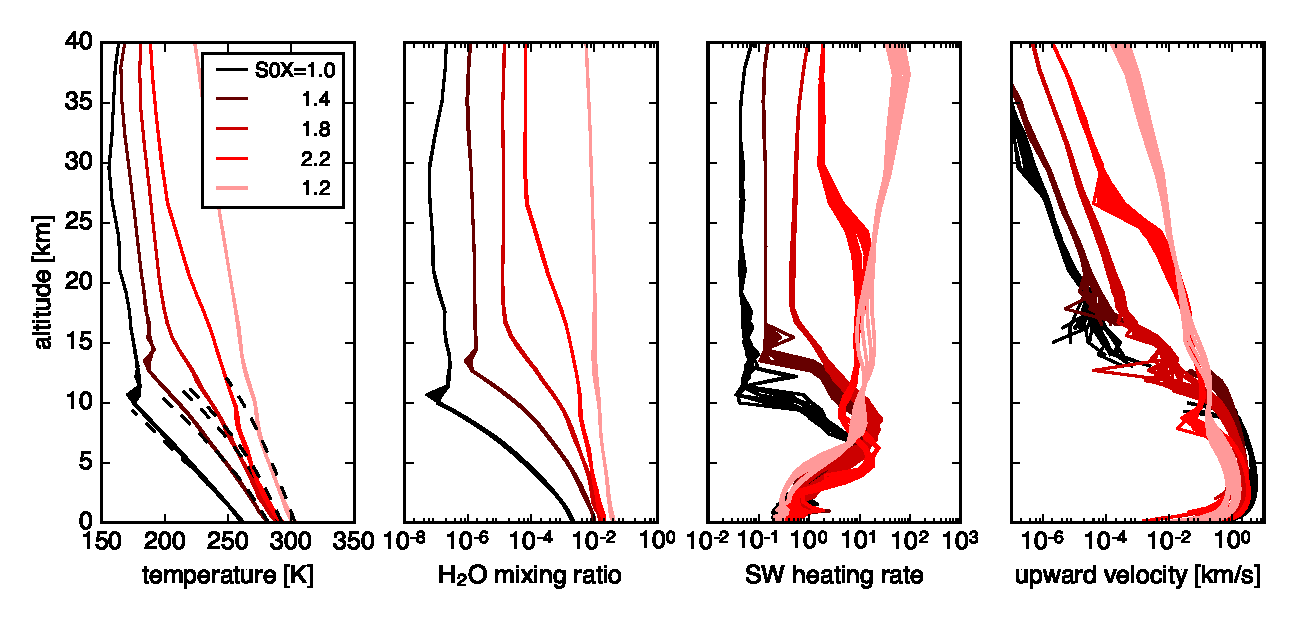
\includegraphics[width=0.8\hsize]{fig/AqOH0TLS_GJ876_temp_xH2O_vz_heat.eps}
    \end{center}
\caption{From left to right, the vertical profiles of temperature, \water mixing ratio, short-wave heating rate, and upward velocity, averaged over the sub-stellar point within the distance of $0.2R_{\oplus }$, for a planet around GJ876 with varying total incident flux. }                                                                                                             
\label{fig:AqOH0TLS_GJ876_temp_xH2O_vz_heat}
\end{figure*}
%%%%%%%%%%%%%%%%%%%%%%%%%%%%%%%%%%%

The development of the large-scale circulation can be naturally explained as follows. 
When the water vapor increases in the upper atmosphere, the heating rate increases due to the stronger absorption by water vapor. 
The air will then react by rising and adiabatically cooling according to the continuity equation for the potential temperature $\Theta $:
%%%
\begin{equation}
\frac{d\Theta }{dt} + ( {\bf v} \cdot \nabla ) \, \Theta = Q_r + Q_l, \label{eq:conserv_energy}
\end{equation}
%%%
or
%%%
\begin{equation}
\frac{d\Theta }{dt} + u \frac{d\Theta }{dx} + v \frac{d\Theta }{dy} + \omega \frac{d\Theta }{dp} = Q_r + Q_l. \label{eq:conserv_energy_2}
\end{equation}
%%%
where $Q_r$ and $Q_l$ are the radiative and latent heatings, $\{ u, v, \omega \}$ is the conventional velocity components toward east ($x-$axis), toward north ($y-$axis), and vertical ($z-$axis; $\omega \equiv  dp/dt$), respectively. 
The latent heating, $Q_l$, is in most cases negligible compared to radiative heating \memo{?}, so it is dropped in the following. 
Likewise, around the sub-stellar point, the vertical motion may be expected to dominate over the horizontal motion, thus second and the third terms in equation (\ref{eq:conserv_energy_2}) may be dropped as an approximation. 
Then, the increase of heating rate, $Q_r$, have an effect of increasing the fourth term. 
Because that the upper atmosphere is stable against convection, i.e., $d \Theta / d p < 0 $, so with larger (positive) $Q_r$ leads to a larger absolute value (with negative sign) for $\omega $, which means the upward motion develops. 
This upward motion of the atmosphere transports water vapor from moist lower atmosphere to upper atmosphere, lowering the slope of water vapor and increasing the moisture in the high altitude, further increasing the absorption by water. 
This interplay between the radiative heating and water vapor transport eventually finds the steady states where $d\Theta/dt = 0$, leaving the steady circulation in the upper atmosphere around the sub-stellar points. 

This positive feedback of \water mixing ratio in the upper atmosphere would make slight difference in the initial radiation field result in order-of-magnitude increase of water vapor. 
As a result, even though the surface temperature is modest, the upper atmosphere gains moisture.  

This picture suggests that the driving factor is the incident flux that reacts with water vapor efficiently, which is near-infrared part of incident flux. 
Indeed, as shown in Figure \ref{fig:qOH0TLS_FNIR_xH2O_247mbar}, a good correlation is found between the \water ratio in the upper atmosphere and the near-infrared portion of the incident flux, integrated over 0.9-3 $\mu {\rm m}$ (the interval is somewhat arbitrary), insensitively to the stellar spectral types. 
This 

%%%%%%%%%%%%%%%%%%%%%%%%%%%%%%%%%%%
\begin{figure}[!h]
    \begin{center}
    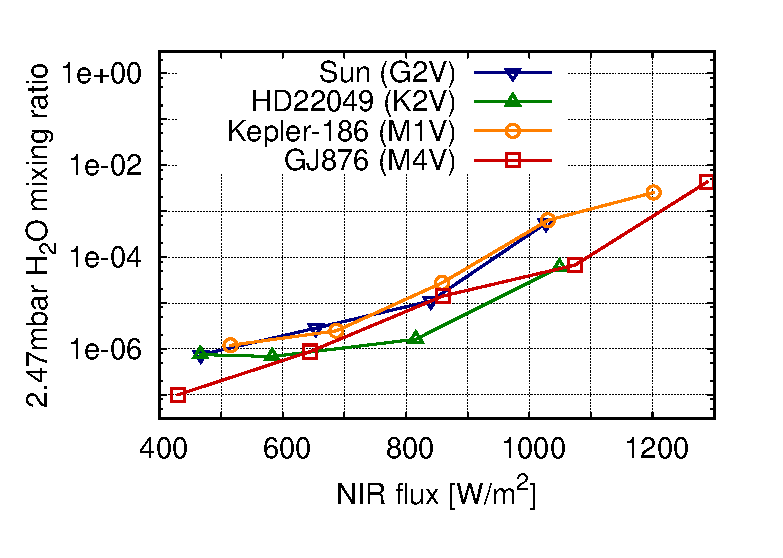
\includegraphics[width=\hsize]{fig/AqOH0TLS_FNIR_xH2O_247mbar.eps}
    \end{center}
\caption{Water mixing ratio at \preslevel ~mbar as a function of the near-infrared portion of the incident flux, integrated over 0.9-3.0 $\mu $m. }                                                                                                             
\label{fig:qOH0TLS_FNIR_xH2O_247mbar}
\end{figure}
%%%%%%%%%%%%%%%%%%%%%%%%%%%%%%%%%%%

%%%%%%%%%%%%%%%%%%%%%%%%%%%%%%%%%%%%%%%%%%%%
\subsection{Transmission Spectra}
\label{ss:result_TransmissionSpectra}
%%%%%%%%%%%%%%%%%%%%%%%%%%%%%%%%%%%%%%%%%%%%

%%%%%%%%%%%%%%%%%%%%%%%%%%%%%%%%%%%
\begin{figure}[!h]
    \begin{center}
    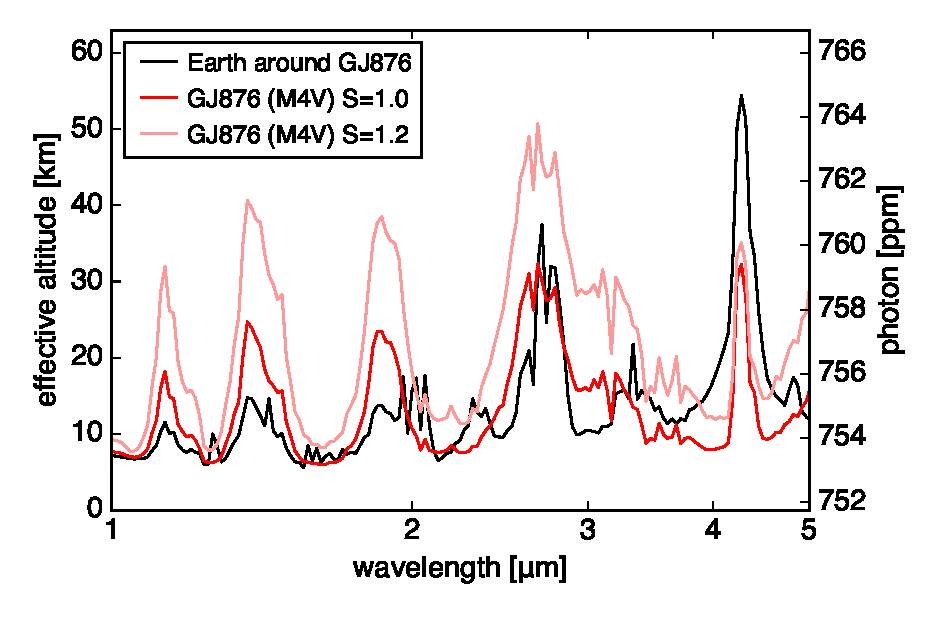
\includegraphics[width=\hsize]{fig/transmission.eps}
    \end{center}
\caption{}                                                                                                             
\label{fig:transmission}
\end{figure}
%%%%%%%%%%%%%%%%%%%%%%%%%%%%%%%%%%%


%%%%%%%%%%%%%%%%%%%%%%%%%%%%%%%%%%%%%%%%%%%%%%%%%%%%%%%%%%%%%%%%%%%
\section{Sensitivity to varying parameters}
\label{s:sensitivity}
%%%%%%%%%%%%%%%%%%%%%%%%%%%%%%%%%%%%%%%%%%%%%%%%%%%%%%%%%%%%%%%%%%%

%%%%%%%%%%%%%%%%%%%%%%%%%%%%%%%%%%%%%%%%%%%%
\subsection{Effect of Ocean Model}
\label{ss:sensitivity_ocean}
%%%%%%%%%%%%%%%%%%%%%%%%%%%%%%%%%%%%%%%%%%%%

So far, we have presented the results using fully-dynamic ocean. 
Instead of calculating the full dynamics of the ocean, it is also possible to assume so-called ``slab'' ocean model \memo{explanation}. 
The slab ocean, the equilibration time can be much shorter; with our configurations, the models equilibrate in $\sim $ 30 Earth years. 
Indeed slab ocean treatment has been regularly used in the published work of 3-dimensional atmospheric modeling for exoplanets. 
Therefore, we checked whether our results is sensitive to the treatment of ocean by comparing our fiducial results with those using ''slab'' ocean model. 

The calculation of the dynamics and thermal properties of ocean is an issue of GCM simulations, because the full treatment of dynamics of ocean requires a significant amount of time (\memo{give some numbers}) to equilibrate \memo{why?}. 



Thus, we 

\begin{itemize}
\item Likely Conclusion: \water mixing ratio is not so sensitive to the ocean model (dynamic ocean v.s. q-flux ocean with zero ocean heat transport).  
\end{itemize}


%%%%%%%%%%%%%%%%%%%%%%%%%%%%%%%%%%%
\begin{figure}[!h]
    \begin{center}
    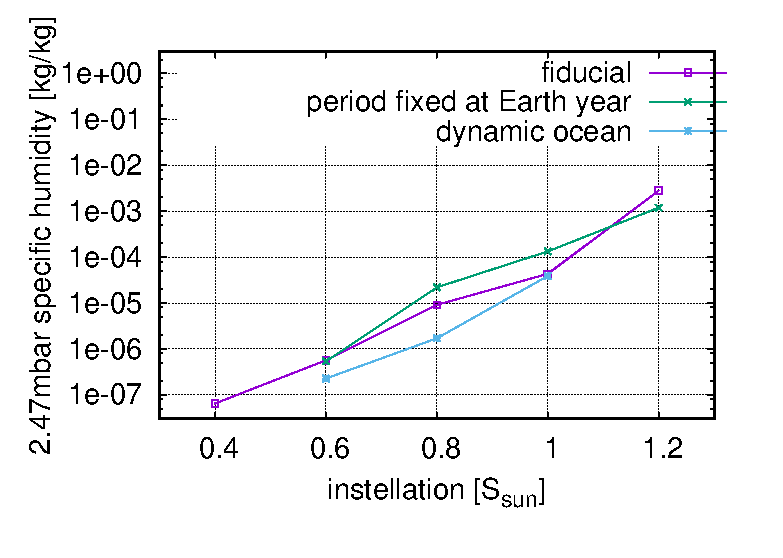
\includegraphics[width=\hsize]{fig/AqOH0TLS_GJ876_q_sensitivity_changeS0X.eps}
    \end{center}
\caption{}                                                                                                             
\label{fig:change_ocean}
\end{figure}
%%%%%%%%%%%%%%%%%%%%%%%%%%%%%%%%%%%



%%%%%%%%%%%%%%%%%%%%%%%%%%%%%%%%%%%%%%%%%%%%
\subsection{Effect of Orbital Period}
\label{ss:sensitivity_Porbit}
%%%%%%%%%%%%%%%%%%%%%%%%%%%%%%%%%%%%%%%%%%%%

\begin{itemize}
\item Conclusion: the orbital period has the secondary effect. Cite \citet{Yang2013}, \citet{Kopparapu2016}. 
\end{itemize}

%%%%%%%%%%%%%%%%%%%%%%%%%%%%%%%%%%%
\begin{figure}[!h]
    \begin{center}
    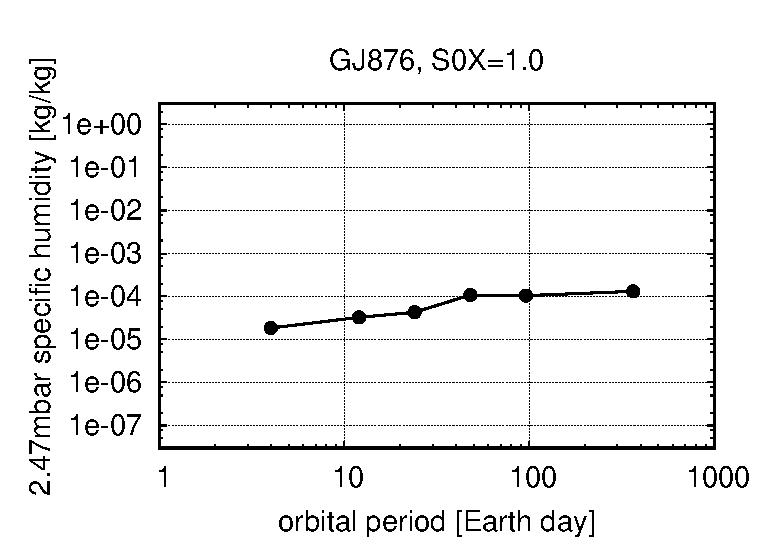
\includegraphics[width=\hsize]{fig/AqOH0TLS_GJ876_q_sensitivity_changeP.eps}
    \end{center}
\caption{}                                                                                                             
\label{fig:changeP}
\end{figure}
%%%%%%%%%%%%%%%%%%%%%%%%%%%%%%%%%%%



%%%%%%%%%%%%%%%%%%%%%%%%%%%%%%%%%%%%%%%%%%%%%%%%%%%%%%%%%%%%%%%%%%%
\section{Summary and Discussion}
\label{s:summary}
%%%%%%%%%%%%%%%%%%%%%%%%%%%%%%%%%%%%%%%%%%%%%%%%%%%%%%%%%%%%%%%%%%%

\acknowledgments

\bibliography{GCM_qstrato_ref}


\appendix


%%%%%%%%%%%%%%%%%%%%%%%%%%%%%%%%%%%%%%%%%%%%%%%%%%%%%%%%%%%%%%%%%%%
\section{Validation of radiation scheme used in our GCM}
\label{ap:radiation}
%%%%%%%%%%%%%%%%%%%%%%%%%%%%%%%%%%%%%%%%%%%%%%%%%%%%%%%%%%%%%%%%%%%

In this paper, we applied a GCM named ROCKE-3D to planets around the stars with different spectral types. 
In doing so, a special caution needed to be taken regarding the accuracy of the radiative transfer calculation, because the baseline model of ROCKE-3D has been developed for the Earth, and the radiative transfer calculation was optimized for solar insolation. 

In order to check the accuracy of the radiative transfer calculation used in GCM model, we compare it with the more accurate high-resolution calculation assuming the same (1-dimensional) atmospheric profile. 
The atmospheric profile to test was the one at the sub-stellar point of a planet around GJ876 with $S_X=1.2$, 
This profile was chosen because of its extremely high \water mixing ratio, which is very different from the Earth. 
Assuming that profile, we calculated short wave radiative transfer with 6 bands (used in GCM) and with 280 bands, both for the cases of solar incident flux and the incident flux of GJ876. 

\memo{David, did you sort out the issue of the water vapor continuum?}

The difference between low- and high- resolution calculation is shown in Figure \ref{fig:socrates}. 
In general, we find a reasonable accuracy of the low-resolution calculation used in GCM; the fractional difference of the upward/downward flux is 4 \% at the maximum (short-wave upward flux) and that of the heating rate is 8\% at the maximum. 

\memo{David, will you describe here better? Will we specifically discuss the concerns others may have, e.g., the weight of the k-coefficient?}

%%%%%%%%%%%%%%%%%%%%%%%%%%%%%%%%%%%
\begin{figure*}[!htb]
    \begin{center}
    \includegraphics[width=0.8\hsize]{fig/rad_comparison_AqOH0TLS_GJ876S12P21L40Q.pdf}
    \includegraphics[width=0.8\hsize]{fig/rad_comparison_diff_AqOH0TLS_GJ876S12P21L40Q.pdf}
    \end{center}
\caption{}                                                                                                             
\label{fig:socrates}
\end{figure*}
%%%%%%%%%%%%%%%%%%%%%%%%%%%%%%%%%%%

%%%%%%%%%%%%%%%%%%%%%%%%%%%%%%%%%%%
%\begin{figure*}[!htb]
%    \begin{center}
%    \includegraphics[width=0.8\hsize]{rad_comparison_AqOH0TLS_GJ876S12P21L40Q.eps}
%    \includegraphics[width=0.8\hsize]{rad_comparison_diff_AqOH0TLS_GJ876S12P21L40Q.pdf}
%    \end{center}
%\caption{}                                                                                                             
%\label{fig:}
%\end{figure*}
%%%%%%%%%%%%%%%%%%%%%%%%%%%%%%%%%%%



\end{document}


